\documentclass[12pt,a4paper]{article}
\bibliographystyle{alphadin}
%\usepackage[onehalfspacing]{setspace}
\usepackage{minted}
\usepackage{url}
\usepackage{graphicx}
\title{Multiplication of Two Bignums on a Nvidia Graphic Card}
\author{Johannes H\"abe  \\
	jh-191149@hs-weingarten.de
	\and 
	Maximilian Nestle \\
	mn-192181@hs-weingarten.de \\\\
	Ravensburg-Weingarten University of Applied Sciences
	}

\date{\today}
% Hint: \title{what ever}, \author{who care} and \date{when ever} could stand 
% before or after the \begin{document} command 
% BUT the \maketitle command MUST come AFTER the \begin{document} command! 
\begin{document}
\maketitle
%
\begin{abstract}
This paper is about testing the performance of the NVIDIA CUDA Fast Fourier Transform library (cuFFT) by multiplying large numbers (bignums) on the graphics card. The performance is measured up to the size of 28000 bits for each factor. The factors are also multiplied on the CPU using the Karatsuba algorithm. For the multiplication of two bignums, performance of the CPU turned out to be in average about one hundred times faster than multiplication on the GPU. The reason for that is, that the preparation (allocation of VRAM, copying data to VRAM) for the multiplication on the GPU is too expensive for only multiplying two factors of the size of 28000 bits. Even taking only the measured times for the pure multiplication, the GPU is still slower than the CPU. By increasing size of the factors from 24 bit up to 28000 bits, the measured times between CPU and GPU are getting closer to each other.
\end{abstract}

\section{Introduction}
The fast multiplication of two large prime numbers is necessary in some procedures to attack asymmetrical encryption algorithms like the RSA encryption. These computations are normally made on the CPU. Classical approaches have $O(n^2)$ complexity, but polynomial multiplication with FFT has $O(nlogn)$ complexity \cite{bantikyan2014big}. Within this paper, General Purpose Computing On GPUs (GPGPU) is used to multiply bignums with the help of the NVIDIA CUDA Fast Fourier Transform library (cuFFT). For this purpose, the computing time of bignum multiplication on CPU and GPU is compared and evaluated in this paper.

\section{Background}
CUFFT Library employs the Cooley-Tukey algorithm to reduce the number of required operations \cite{nvidia2012cuda} resulting in $O(nlogn)$ complexity. 

TODO: fft formeln hier reinballern

\section{Measurement conditions}
For the multiplications an Acer Aspire V3-772G is used. The Acer has got a NVIDIA GTX 850M graphics card and an Intel Core i5 4200M CPU. The graphics card disposes of 2004 MIB storage. The Acer is running the Linux distribution Ubuntu. The code that is used to multiply two bignums on the GPU is using the cuFFT library from NVIDIA. The multiplications on the CPU are done with the \mintinline{c}{BN_mul()} function which is based on the Karatsuba recursive multiplication algorithm \cite{young1995bnmul}. The Karatsuba algorithm has $O(n^{1.585})$ complexity \cite{dietzfelbinger2012eff}. The \mintinline{c}{BN_mul()} function comes with the openssl library.

The computation time for the multiplications of the two numbers is measured up to the size of 28000 bits for each factor. The step size for the multiplications is 24 bits. That means that computations are done for numbers of the size 24 bits, 48 bits, 72 bits and so on. The numbers used for computations are created randomly. To prevent variations because of random created numbers that are easy to multiply, one hundred multiplications, each with random numbers, are done for each step of 24 bits.

\section{Evaluation of the measured times}
For the time measurement the C library function \mintinline{c}{clock(void)} is used. The legend of the measured times is explained in table \ref{Description}. In table \ref{AvgMaxMin} the minimum, maximum and average times for the calculations from 24 bits to 28800 bits are seen. The minimum is for all seven categories located between 24 and 120 bits, the maximum was always close to 28000 bits. It can be derived from the table, that GPU\_Alloc and CUDA\_Pre cost by far the most time. They take each in average about one hundred times more time than the CPU calculation.

\begin{table}
\centering
\caption{Descriptions of the abbreviations of the measured times.}
\vspace{0.5cm}
\label{Description}
\begin{tabular}{p{2cm}|p{9.0cm}|}
\cline{1-2}
 \multicolumn{1}{|l|}{CPU} & The time needed for the multiplications of the two bignums on the CPU using the \mintinline{c}{BN_mul()} function. \\ \hline
 \multicolumn{1}{|l|}{GPU\_All} & The sum of the times needed for GPU\_Alloc, GPU\_Calc, GPU\_Clean, CUDA\_Pre, and CUDA\_Post. \\ \hline
 \multicolumn{1}{|l|}{GPU\_Alloc} & The time needed to allocate the amount of graphics card memory needed for the two bignums using \mintinline{c}{cudaMalloc()} and copying them to the graphics card memory by using \mintinline{c}{cudaMemcpy()}.
 \\ \hline
 \multicolumn{1}{|l|}{GPU\_Calc} & The amount of time needed for the calculation of the two bignums on the GPU. This includes converting the bignums to frequency domain, multiplying them with \mintinline{c}{ComplexPointwiseMulAndScale()} and converting them back to time domain. \\ \hline
 \multicolumn{1}{|l|}{GPU\_Clean} & The sum of the times needed to copy the data back to the host by using \mintinline{c}{cudaMemcpy()} and to free the graphics card memory by using \mintinline{c}{cufftDestroy()} and \mintinline{c}{cudaFree()}.\\ \hline
 \multicolumn{1}{|l|}{CUDA\_Pre} & The time needed to prepare the data for the multiplication. The algorithm needs to convert the two numbers from the datatype bignum to float vectors. Float vectors are required for the \mintinline{c}{cudaMemcpy()} function. Also the size of the vectors needs to be adjusted, because cuFFT saves the solution in one of the initial bignums. \\ \hline
 \multicolumn{1}{|l|}{CUDA\_Post} & The time needed to prepare the result. This includes removing excess zeros, processing carry and turning the result from a float vector to a bignum. \\ \hline
\end{tabular}
\end{table}

\begin{table}
\centering
\caption{Average, minimum and maximum times measured of all bit sizes.}
\vspace{0.5cm}
\label{AvgMaxMin}
\begin{tabular}{p{2cm}|p{3cm}|p{3cm}|p{3cm}|}
\cline{2-4}
 & \multicolumn{3}{l|}{Times in seconds}  \\ \hline 
 \multicolumn{1}{|l|}{} & $Minimum$ & $Maximum$ & $Average$\\ \hline
 \multicolumn{1}{|l|}{CPU} & $1 \times 10^{-6}$ & $9 \times 10^{-5}$ & $4,16 \times 10^{-5}$ \\ \hline
 \multicolumn{1}{|l|}{GPU\_All} & $1,72 \times 10^{-3}$ & $1,48 \times 10^{-2}$ & $7,19 \times 10^{-3}$ \\ \hline
 \multicolumn{1}{|l|}{GPU\_Alloc} & $1,42 \times 10^{-3}$ & $6,13 \times 10^{-3}$ & $3,67 \times 10^{-3}$ \\ \hline
 \multicolumn{1}{|l|}{GPU\_Calc} & $8,7 \times 10^{-5}$ & $4,48 \times 10^{-4}$ & $2,45 \times 10^{-4}$ \\ \hline
 \multicolumn{1}{|l|}{GPU\_Clean} & $1,71 \times 10^{-4}$ & $8,17 \times 10^{-4}$ & $4,23 \times 10^{-4}$ \\ \hline
 \multicolumn{1}{|l|}{CUDA\_Pre} & $8 \times 10^{-6}$ & $6,88 \times 10^{-3}$ & $2,44 \times 10^{-3}$ \\ \hline
 \multicolumn{1}{|l|}{CUDA\_Post} & $2 \times 10^{-6}$ & $9,21 \times 10^{-4}$ & $3,97 \times 10^{-4}$ \\ \hline
\end{tabular}
\end{table}

\begin{figure}[hbt!]
\centering 
\caption{GPU\_Calc (blue) and CPU (red) with computed polynomial.}
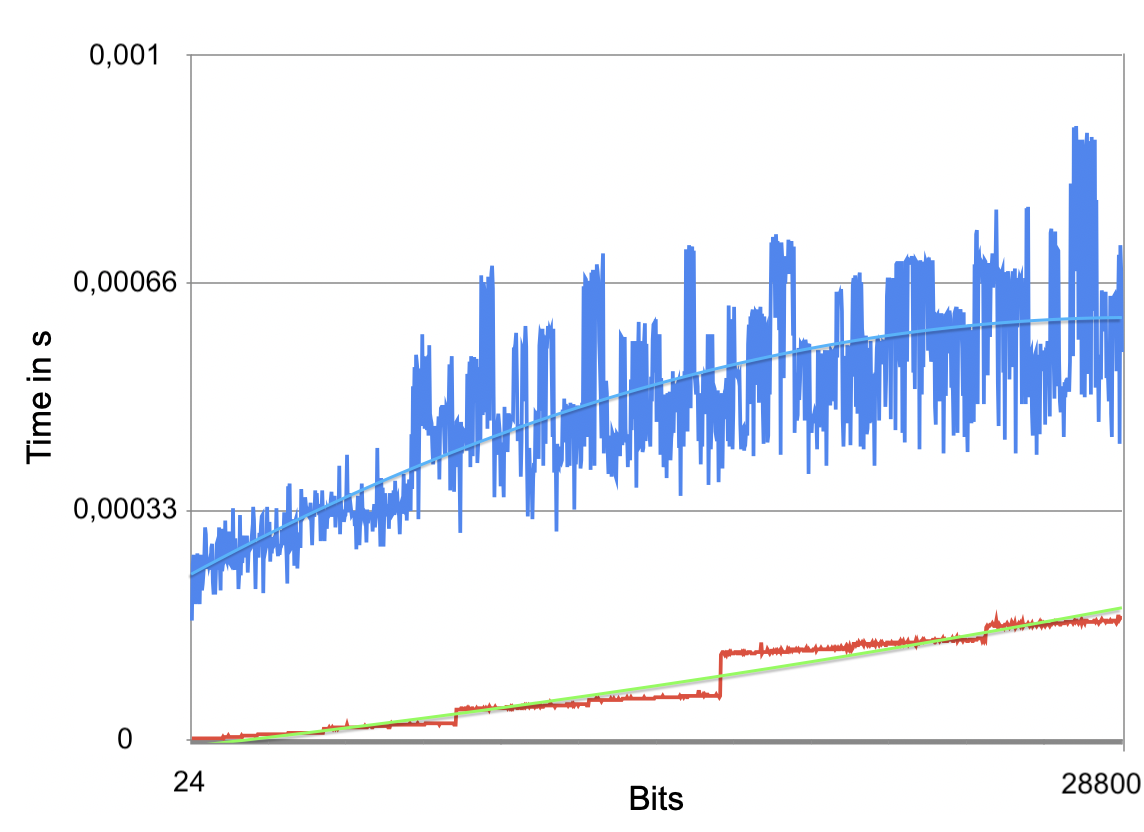
\includegraphics[scale=0.66]{gpucalc_cpu_des.png}
\label{cpugpu_times} 
\end{figure}

 With Numbers by Apple, the second grade polynomial of GPU\_Calc and CPU were computed and visualized in figure \ref{cpugpu_times} with the original graphs. The slope of the blue polynomial ist getting smaller, while the slope of the green polynomial is increasing.

\begin{center}
    $GPU\_Calc_{poly}(x) = -1.269*10^{-10}x^2 + 3.086*10^{-7}x + 0.0001$
\end{center}

\begin{center}
    $CPU_{poly}(x) = 1.77*10^{-11}x^2 + 6.295*10^{-8}x - 4.799*10^{-6}$
\end{center}

From figure \ref{cpugpu_times} it can be derived, that the GPU is getting more effective in comparison to the CPU, the bigger the numbers get. This assumption is only valid as long as we use Karatsuba for CPU and FFT for GPU. The graph reflects the complexities of the algorithms.

The measurements were also done on two more computers, to make sure, that the structure of the resulting graphs is nearly the same and not a specific result of the depending hardware of the computers. The assumption was confirmed.

\section{Conclusion}
The big issues are that the times needed for preparation and allocation of the GPU are totally out of range. The CPU is able to store all data in cache, GPU data transfer takes too long \cite{cooper2011gpu}. Even if only the calculation process on the GPU with the CPU are compared, the CPU is up to 28000 bits still at least 5 times faster than the GPU. With parallel computing of multiple pairs of numbers on the GPU, it can be assumed that the process can be accelerated, for example by allocating a bigger amount of VRAM and putting multiple pairs of numbers on the graphics card memory with just one call of \mintinline{c}{cudaMemcpy()}.

The time measurements lead to the conclusion, that multiplying only one pair of numbers on a GPU with cuFFT is way too inefficient, computing them on the CPU is the recommended way. An exception could be mulitplying numbers that are way bigger than 28000 bits, because the larger the numbers get, the more effective becomes the multiplication on the GPU. Although more performance improvement experiments would be needed to confirm the assertion.

\bibliography{literatur}

\end{document}
